\documentclass[12pt]{article}
  
  \usepackage{article}
  
  \usepackage{graphicx,url}
  
  \usepackage[brazilian]{babel}
  \usepackage[utf8]{inputenc}
  \usepackage[T1]{fontenc}
  \usepackage{lipsum}
  
  
  \sloppy
  
  \title{Arquiteturas e modelos da computação em nuvem móvel: uma revisão sistemática}
  
  \author{Victor H. Fernandes\inst{1}, Marcelo M. Oliveira\inst{1}, Lucas M. \inst{1}}
  
  
  \address{Universidade de Brasília (UNB) - Campus FGA
  \\ Gama - DF - Brasil
  \email{\{victor.hmfd,martins.oliveira.mo,lucasamartins465\}@gmail.com}
  }
  
\begin{document}

\maketitle

\begin{resumo}
  A computação em nuvem móvel (MCC) é um conceito bastante novo, porém de grande impacto nas experiências de usabilidade
  dos usuários móveis, fornecendo a esses usuários, os serviços de processamento e armazenamento de dados nas nuvens.
  Os dispositivos móveis não precisam mais de uma configuração poderosa (por exemplo, velocidade da CPU e capacidade de memória)
  porque todos os módulos de computação complicados podem ser processados nas nuvem. Porém, por ser um conceito relativamento novo,
  ainda traz alguns desafios. Sendo assim, neste artigo, é apresentado uma revisão sistemática a cerca  das arquiteturas e modelos da
  computação em nuvem móvel, afim de investigar quais são os principais desafios da computação em nuvem em aplicativos móveis.
\end{resumo}

\begin{itemize}
  \item \textit{\textbf{Palavras-chave:} modelos de computação em nuvem em dispositivos movéis, Modelos MCC, modelos de nuvem em dispositivos
  movéis, arquitetura de nuvem em dispositivos movéis, computação em nuvem em dispositivos movéis, MCC, computação em dispositivos
  movéis, revisão da literatura na nuvem em dispositivos movéis, desafios de nuvem em dispositivos movéis, desafios.}
\end{itemize}

\begin{abstract}
  Mobile cloud computing (MCC) is a fairly new concept, but it has a major impact on the usability experiences
  of mobile users, providing these users with the services of processing and storing data in the clouds. Mobile devices
  no longer need a powerful configuration (for example, CPU speed and memory capacity) because all complicated computing
  modules can be processed in the cloud. However, because it is a new concept, it still has some challenges. In this article,
  a systematic review is presented about the architectures and models of mobile cloud computing, in order to investigate the
  main challenges of cloud computing in mobile applications.
\end{abstract}

\begin{itemize}
  \item \textit{\textbf{Keywords:} mobile cloud computing models, MCC models, mobile cloud models, mobile cloud architecture, mobile cloud
  computing, MCC, mobile computing, mobile cloud literature review, mobile cloud challenges, challenges}
\end{itemize}




\section{Introdução}

\lipsum[1]

\section{Referencial Teórico}

Nesta seção é apresentado os conceitos da computação em nuvem e da computação em nuvem
móvel, bem como seus modelos e arquiteturas.

\subsection{Computação em Nuvem}

A computação em nuvem, descrita pela entidade americana NIST (Instituto Nacional de Padrões e Tecnologia)
como uma plataforma \textit{user friendly}, ou seja, possui uma interação facilitada com o usuário, que permite o
acesso de recursos computacionais compartilhados sob demanda \cite{alizadeh2013}.

Essa tecnologia consiste em um \textit{cluster} de servidores e computadores pessoais conectados com o objetivo de
prover inúmeros serviços, sejam eles de \textit{hardware}, aplicação ou serviços, por meio da internet. Nesse contexto,
Kumar et al. \cite{kumar2014} afirma que a computação em nuvem centraliza todos os recursos computacionais, mas seu
acesso pode se dar em qualquer lugar, a qualquer momento, utilizando a internet como meio.

Outra descrição para computação em nuvem é a integração entre computação como serviço e \textit{software} como serviço,
onde as aplicações estão acessíveis através da internet, e os sistemas de \textit{hardware} e \textit{software} mantidos
pelos \textit{data centers} são providos de modo a serem alcançados remotamente pelos usuários \cite{alizadeh2013}.

O conceito de nuvem pode ser ligado ao advento dos \textit{mainframes} de larga escala na década de 1950,
onde esses equipamentos, vistos como o futuro da computação, eram vastamente utilizados na academia e em
grandes corporações. Mais tarde, na década de 1990, companhias de telecomunicação começaram a fornecer
serviços de rede privada virtual (VPN) com qualidade equivalente e custos bem mais baixos.
Evoluções tecnológicas continuaram acontecendo até que em 2008 o \textit{Eucalyptus} surgiu como
a primeira plataforma \textit{open-source} para a implementação de nuvens privadas. Atualmente,
grandes corporações como Google, Amazon, Microsoft, entre outras, estão se empenhando na criação de nuvens mais
eficientes, seguras, confiáveis e rentáveis \cite{kumar2014}.

Na computação em nuvem, todos os recursos formam um \textit{cloud resource pool} (agrupamento
de recursos em nuvem, em uma tradução livre), e então são alocados
dinamicamente para diferentes aplicações e serviços. Além disso, o uso da virtualização
permite que vários serviços,  sistemas operacionais e aplicações possam ser executados
em um servidor compartilhado. Isso possibilita que, quando um servidor esteja sobrecarregado,
a instancia destes sistemas operacionais e aplicações possam ser transportadas para
um servidor vago dentro do \textit{cloud resource pool}. Neste modelo, o
processamento local e recursos de armazenamento são transferidos para a nuvem.
Assim, os usuários corporativos não precisam adquirir grandes centrais de computação
local e contratar mão de obra especializada. Os recursos são disponibilizados sob
demanda, em um esquema de pagamento por uso. Este sistema beneficia, principalmente,
pequenas empresas \cite{jing2010}.

Segundo Jing e Jian-jun \cite{jing2010} a computação em nuvem possui três
características básicas:

\begin{itemize}
  \item Ao contrário das infraestruturas de hardware convencionais, a computação
  em nuvem é composta por um grande número de servidores distribuídos de baixo
  custo.
  \item O desenvolvimento das plataformas de computação em nuvem é colaborativo
  para proporcionar uma maior utilização de recursos. Deste modo, a construção
  das aplicações é melhorada.
  \item Falhas entre os múltiplos servidores do sistema devem ser levados em
  consideração ao se projetar o software.
\end{itemize}

Já Alizadeh e Hassan \cite{alizadeh2013} afirmam que a computação em nuvem possui três
modelos de arquitetura, quatro modelos de implementação e cinco aspectos chave. São eles:

\subsection{Aspectos chave da Computação em Nuvem}

\begin{itemize}
  \item \textbf{On-demand Self-service:} Se um usuário necessitar de uma requisição particular
  com urgência, que necessite de um determinado recurso computacional, em um determinado
  espaço de tempo, que possa envolver armazenamento de dados, uso de software, tempo de CPU
  etc, a plataforma deve ser capaz de fornecer este recurso sem a necessidade de um provedor.
  \item \textbf{Acesso amplo à rede:} Os recursos podem ser facilmente obtidos da rede utilizando
  um conjunto de protocolos que usam plataformas heterogêneas, como computadores pessoais,
  dispositivos móveis, entre outros.
  \item \textbf{Agrupamento de Recursos:} O provedor da infraestrutura deve disponibilizar várias
  ferramentas para computação que possam ser utilizadas de maneira robusta por muitos usuários.
  Estas ferramentas provêm flexibilidade por possibilitar o gerenciamento da utilização de recursos.
  \item \textbf{Elasticidade Rápida:} Os recursos disponíveis devem ser rapidamente
  expandidos e fornecidos para atender uma grande demanda. Os usuários enxergam estes
  recursos como infinitos, podendo ser adquiridos a qualquer momento.
  \item \textbf{Serviços Quantificados:} A utilização de serviços é quantificada e
  monitorada continuamente, o que permite a otimização da utilização dos recursos,
  o fornecimento de relatórios para os usuários e a utilização do modelo de negócio
  \textit{pay-per-use} (pague por uso).
\end{itemize}

\subsection{Modelos Arquiteturais da Computação em Nuvem}

\begin{figure}[ht]
  \centering
  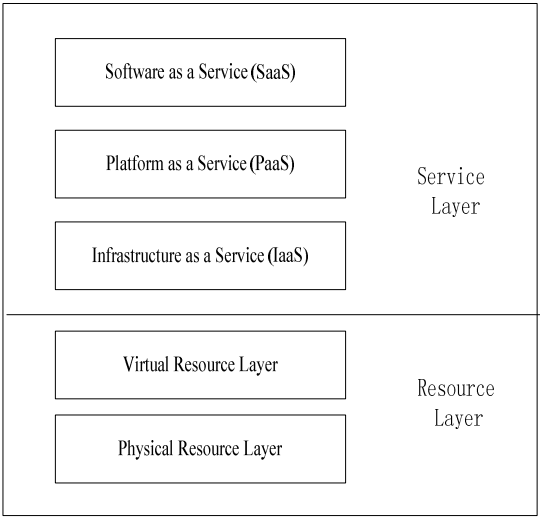
\includegraphics[scale= 0.5]{figuras/camadasCC.png}
  \caption{Arquitetura da Computação em Nuvem}
  \label{camadasCC}
\end{figure}

Em geral, a arquitetura de computação em nuvem é dividida em duas camadas, como
exemplificado na figura \ref{camadasCC}: A camada mais baixa é baseada na virtualização
de recursos de armazenamento e processamento. Já a camada superior provê os serviços
específicos da computação em nuvem \cite{jing2010}. Esta camada é dividida em IaaS, PaaS e Saas:

\begin{itemize}
  \item \textbf{Infraestrutura como Serviço (IaaS):} Camada que fornece ao usuário
  a possibilidade de executar tarefas de processamento, armazenamento, comunicação,
  entre outros recursos solicitados com o objetivo de executar sistemas operacionais e
  aplicações. Os usuários não tem contato com a camada física, mas pode controlar a
  utilização dos recursos.
  \item \textbf{Plataforma como Serviço (PaaS):} Camada que suporta o \textit{design}
  e o desenvolvimento de aplicações, testes, implementação e hospedagem. Permite
  a utilização de memória, servidores, plataformas, serviços, e a hospedagem de aplicações
  como Google AppEngine, AppExchange, entre outras.
  \item \textbf{\textit{Software} como Serviço (SaaS):} Camada que disponibiliza
  aplicações sob demanda, que podem ser acessadas por diversos usuários ou organizações
  ao mesmo tempo por meio da internet. Esta camada elimina a necessidade de instalar e
  executar um \textit{software}, e os custos com manutenção e suporte. Exemlos de SaaS são
  Google Drive, Gmais, entre outros.
\end{itemize}

\subsection{Modelos de Implementação da Computação em Nuvem}

\begin{itemize}
  \item \textbf{Nuvem Pública:} Neste modelo, os provedores oferecem os recursos
  em forma de serviços aos usuários. As nuvens públicas são vantajosas para os provedores,
  pois não envolvem investimentos financeiros, e os riscos são responsabilidade do
  fornecedor da infraestrutura.
  \item \textbf{Nuvem Privada:} Nesta modalidade de nuvem, os serviços e recursos são
  gerenciados e acessados por uma organização específica. O acesso às informações
  são limitados a usuários membros dessa organização. A vantagem desse modelo é a segurança
  e a privacidade dos dados, que, geralmente, é superior.
  \item \textbf{Nuvem Hibrida:} É a combinação entre dois ou mais modelos de nuvem.
  Empresas utilizam a nuvem híbrida para mover processos não essenciais, enquanto mantém
  os processos centrais e urgentes na nuvem privada.
  \item \textbf{Nuvem Comunitária:} Modelo que permite que várias organizações, que
  utilizam as mesmas tecnologias, propostas e políticas, trabalharem juntas utilizando
  políticas, recursos e infraestruturas semelhantes, o que reduz custos operacionais e
  proporciona um melhor gerenciamento de recursos.
\end{itemize}

\subsection{Computação em Nuvem Móvel}

Aepona \cite{aepona2010} descreve a computação em nuvem móvel ou MCC(Mobile Cloud Computing) como um novo paradigma para aplicações
móveis pelo qual o processamento e armazenamento de dados são movidos do dispositivo móvel para plataformas de computação
poderosas e centralizadas, localizadas em nuvens. Esses aplicativos são então acessados através da conexão sem fio com base em
um cliente ou navegador web nativo nos dispositivos móveis.

Resumidamente, o MCC fornece aos usuários móveis os serviços de processamento e armazenamento de dados nas nuvens.
Os dispositivos móveis não precisam de uma configuração poderosa (por exemplo, velocidade da CPU e capacidade de memória)
porque todos os módulos de computação complicados podem ser processados nas nuvens \cite{liu2010}.

De acordo com Atta \cite{atta2013}, o principal objetivo da computação em nuvem é facilitar as pequenas empresas,
de forma econômica, fornecendo acesso a tecnologias que estão além do alcance deles. Ao usar a computação em nuvem,
as pequenas empresas podem expandir seus recursos de TI com base em demandas de serviço e aproveitar oportunidades
de crescimento para competir com outras empresas dentro do mercado.

Alternativamente, o principal objetivo da computação em nuvem móvel é fornecer experiências de usuários aprimoradas
aos usuários mobile que podem ser, em termos de tempo de computação, vida útil da bateria, comunicação, serviços e
aprimoramento de recursos de dispositivos móveis.

Portanto, ambas as tecnologias têm objetivos e desafios diferentes. Por exemplo, na computação em nuvem móvel,
a conectividade de rede, a quantidade de comunicação, o custo de utilização da largura de banda e a energia do
dispositivo móvel são considerados os principais problemas, o que pode não ser o caso na computação em nuvem.

No entanto, os modelos de aplicativos de nuvem móvel são baseados no modelo de serviço padrão da nuvem que inclui
Infraestrutura como Serviço (IaaS), Plataforma como um serviço (PaaS) e Software as a Service (SaaS). Portanto,
com base no funcionamento dos modelos de aplicativos, qualquer uma dessas camadas de serviço pode ser utilizada.
Alguns dos serviços bem conhecidos para computação em nuvem móvel incluem Amazon Elastic Compute Cloud (EC2) \cite{amazon},
Google App Engine \cite{googleapp} e Microsoft Azure \cite{azure}.

Atta \cite{atta2013} diz que não existe uma definição padrão ou caracterização de recursos da computação em nuvem móvel.
Portanto, apresenta uma comparação possível de computação em nuvem e computação em nuvem móvel, em termos de significância
das questões listadas conforme tabela \ref{comparisonClouds}.

% ######## init table ########
\begin{table}[h]
  \centering
  % distancia entre a linha e o texto
  {\renewcommand\arraystretch{1.25}
  \begin{tabular}{ l l l }
    \cline{1-1}\cline{2-2}\cline{3-3}
    \multicolumn{1}{|c|}{\textbf{Questões}} &
    \multicolumn{1}{c|}{\textbf{Computação em nuvem}} &
    \multicolumn{1}{c|}{\textbf{Computação em nuvem móvel}}
    \\
    \cline{1-1}\cline{2-2}\cline{3-3}
    \multicolumn{1}{|c|}{Energia do dispositivo} &
    \multicolumn{1}{c|}{x} &
    \multicolumn{1}{c|}{ok}
    \\
    \cline{1-1}\cline{2-2}\cline{3-3}
    \multicolumn{1}{|c|}{Custo de utilização da banda} &
    \multicolumn{1}{c|}{x} &
    \multicolumn{1}{c|}{ok}
    \\
    \cline{1-1}\cline{2-2}\cline{3-3}
    \multicolumn{1}{|c|}{Conectividade de rede} &
    \multicolumn{1}{c|}{x} &
    \multicolumn{1}{c|}{ok}
    \\
    \cline{1-1}\cline{2-2}\cline{3-3}
    \multicolumn{1}{|c|}{Mobilidade} &
    \multicolumn{1}{c|}{x} &
    \multicolumn{1}{c|}{ok}
    \\
    \cline{1-1}\cline{2-2}\cline{3-3}
    \multicolumn{1}{|c|}{Largura de Banda} &
    \multicolumn{1}{c|}{x} &
    \multicolumn{1}{c|}{ok}
    \\
    \cline{1-1}\cline{2-2}\cline{3-3}
    \multicolumn{1}{|c|}{Segurança} &
    \multicolumn{1}{c|}{ok} &
    \multicolumn{1}{c|}{ok}
    \\
    \hline
    
  \end{tabular} }
  \caption{Comparação entre computação em nuvem e computação em nuvem móvel}
  \label{comparisonClouds}
\end{table}


\subsubsection{Arquitetura da computação em nuvem móvel}


Na atual arquitetura de nuvem móvel, os dispositivos móveis podem acessar os serviços da nuvem de duas maneiras,
ou seja, através da rede móvel (rede de telecomunicações) ou através de pontos de acesso, conforme mostrado na Figura \ref{arquiteturaMCC}.

\begin{figure}[ht]
  \centering
  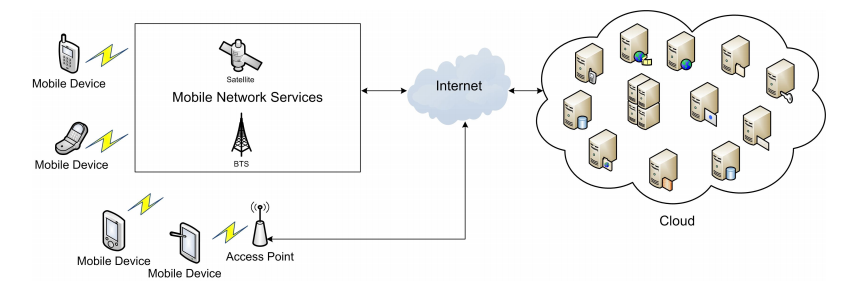
\includegraphics[scale= 0.5]{figuras/arquiteturaMCC.png}
  \caption{Arquitetura da computação em nuvem móvel}
  \label{arquiteturaMCC}
\end{figure}

No caso da rede móvel (provedor de rede de telecomunicações), os dispositivos móveis, como os celulares smartphones \cite{satelite},
estão conectados a uma rede móvel através de uma Estação Base (BS) ou através de um link de satélite. No entanto,
se os smartphones não estiverem equipados com um módulo de comunicação por satélite, são utilizados dispositivos
externos de comunicação por satélite \cite{spot}. As redes de telecomunicações estão mais conectadas à Internet e
fornecem conectividade com a Internet aos usuários. Portanto, se os usuários tiverem conectividade de rede móvel,
os usuários podem acessar serviços baseados em nuvem através da Internet.

No caso do ponto de acesso, os usuários móveis se conectam aos pontos de acesso através do Wi-Fi, que está mais conectado
ao provedor de serviços de Internet para fornecer conectividade com a Internet aos usuários. Portanto, os usuários da nuvem móvel
podem acessar serviços baseados em nuvem sem utilizar serviços de telecomunicações, o que pode cobrar por tráfego de dados.
Além disso, as conexões baseadas em Wi-Fi oferecem pouca latência e consomem menos energia em comparação com as conexões 3G \cite{cuervo2010}.
Conseqüentemente, usuários da nuvem móvel preferem usar conexões Wi-Fi sempre que acessíveis.

\section{Metodologia}

Para a elaboração deste estudo, foi realizada uma revisão sistemática de literatura,
ou SRL(Systematic Literature Review), de acordo com os critérios e o modelo adotado
por \cite{kitchenham2012}. Para isso, a revisão foi divida em três fases: planejamento,
execução e análise dos resultados, onde cada fase será melhor detalhada nas subseções seguintes.
A fase de Análise dos resultados, por comtemplar a parte principal desse trabalho, será detalhada
na próxima seção.

\subsection{Planejamento}

A fase de planejamento foi dividida em etapas e estão detalhadas nos subtópicos a seguir:

\subsubsection{Questão de pesquisa}

Este estudo responde a seguinte questão de pesquisa:

\begin{itemize}
  \item QP: Quais os principais desafios da computação em nuvem em aplicativos móveis?
\end{itemize}

\subsubsection{Definição da string de busca}

Para obtenção de resultados relevantes a partir das pesquisas a serem realizadas, foi necessário a criação de uma string de busca.
Para a criação dessa string, foi utilizado o método PICO(Population, Intervention, Comparison, Output), que foi
proposto por \cite{SANTOS2007}. O método PICO é uma maneira de facilitar o entendimento da questão de pesquisa, transformando-a
em uma string de busca.

A tabela \ref{pico} mostra como o método PICO foi definido.


\begin{table}[h]
  \centering
  % distancia entre a linha e o texto
  {\renewcommand\arraystretch{1.25}
  \begin{tabular}{ l l }
    \cline{1-1}\cline{2-2}
    \multicolumn{1}{|p{5cm}|}{Elemento PICO} &
    \multicolumn{1}{p{8cm}|}{Argumento}
    \\
    \cline{1-1}\cline{2-2}
    \multicolumn{1}{|p{5cm}|}{P (Population)} &
    \multicolumn{1}{p{8cm}|}{mobile cloud computing}
    \\
    \cline{1-1}\cline{2-2}
    \multicolumn{1}{|p{5cm}|}{I (Intervention)} &
    \multicolumn{1}{p{8cm}|}{mobile cloud computing models, mobile cloud models, mobile cloud architecture, MCC}
    \\
    \cline{1-1}\cline{2-2}
    \multicolumn{1}{|p{5cm}|}{C (Comparison)} &
    \multicolumn{1}{p{8cm}|}{não se aplica}
    \\
    \cline{1-1}\cline{2-2}
    \multicolumn{1}{|p{5cm}|}{O (Outcome)} &
    \multicolumn{1}{p{8cm}|}{mobile cloud literature review, mobile cloud challenges, challenges}
    \\
    \hline
  \end{tabular} }
  \caption{Definição da string de busca utilizando o método PICO}
  \label{pico}
  
\end{table}

Com os principais argumentos que abordam a questão de pesquisa deste estudo, foi possível a confecção da string de busca,
para uma busca mais precisa sobre o tema. Abaixo segue a primeira string definida:

(“mobile cloud computing models” OR “MCC models”) AND ("Mobile cloud models") AND ("Mobile cloud architecture") AND (“Mobile
cloud computing” OR “MCC”)

Após um refinamento da string acima, foi elaborada outra string com mais argumentos, que nos possibilitou uma maior precisão
sobre o matérial encontrado
para a escrita desta SRL. Abaixo segue a segunda string definida:

(“mobile cloud computing models” OR “MCC models”) AND ("Mobile cloud models") AND ("Mobile cloud architecture") AND (“Mobile
cloud computing” OR “MCC”) AND (“mobile computing”) AND (“mobile cloud literature review”) AND (“mobile cloud challenges”) AND
(“challenges”)

\subsubsection{Bases de busca}

Com a string de busca montada, definiu-se as bases de busca que nos retornaram artigos para a escrita dessa SRL. As bases de
dados utilizadas para as pesquisas foram as seguintes:

\begin{itemize}
  \item IEEE Xplore (http://ieeexplore.ieee.org/Xplore/home.jsp)
  \item ACM Digital Library (https://dl.acm.org/)
  \item SpringerLink (https://link.springer.com/)
  \item ScienceDirect(http://www.sciencedirect.com/)
\end{itemize}

\subsubsection{Critérios}

Para a escolha das publicações foram feitos dois tipos de critérios, critério de inclusão e critério de exclusão.
Esse critérios foram utilizados para que os artigos selecionados fossem relevantes para para compor este estudo.

Critérios de inclusão:

\begin{itemize}
  \item CI1: A publicação deve estar escrita em inglês ou português;
  \item CI2: A publicação deve ter sido publicada a partir de 2005;
  \item CI3: A publicação deve apresentar estudos relevantes ao tema proposto nesta revisão sistemática no abstract.
\end{itemize}

Após selecionar as publicações, foi utilizado o seguinte critério para a exclusão do restante das publicações:

\begin{itemize}
  \item CE1. O abstract da publicação foge do tema proposto.
\end{itemize}

\subsection{Execução}

Após a definição da string de busca, foi realizada a execução da busca nas bases citadas anteriormente. Realizada a
busca e utilizando os critérios de inclusão e exclusão para filtrar as publicações encontradas, foi feita a extração 
dos principais dados para a realização dessa SRL. Através do filtro utilizado a partir dos critérios,
temos a tabela \ref{publicacoes} com a quantidade de publicações relevantes encontradas em cada base:


\begin{table}[h]
  \centering
  % distancia entre a linha e o texto
  {\renewcommand\arraystretch{1.25}
  \begin{tabular}{ l l }
    \cline{1-1}\cline{2-2}
    \multicolumn{1}{|p{4.500cm}|}{\textbf{Base pesquisada}} &
    \multicolumn{1}{p{4.500cm}|}{\textbf{Publicações encontradas}}
    \\
    \cline{1-1}\cline{2-2}
    \multicolumn{1}{|p{4.500cm}|}{\textbf{IEEE Xplore} \centering } &
    \multicolumn{1}{p{4.500cm}|}{7 \centering }
    \\
    \cline{1-1}\cline{2-2}
    \multicolumn{1}{|p{4.500cm}|}{\textbf{ACM Digital Library} \centering } &
    \multicolumn{1}{p{4.500cm}|}{4 \centering }
    \\
    \cline{1-1}\cline{2-2}
    \multicolumn{1}{|p{4.500cm}|}{\textbf{SpringerLink} \centering } &
    \multicolumn{1}{p{4.500cm}|}{2 \centering }
    \\
    \cline{1-1}\cline{2-2}
    \multicolumn{1}{|p{4.500cm}|}{\textbf{ScienceDirect} \centering } &
    \multicolumn{1}{p{4.500cm}|}{1 \centering }
    \\
    \hline
    
  \end{tabular} }
  \caption{Publicações relevantes encontradas} 
  \label{publicacoes} 
\end{table}



\section{Análise dos Resultados}

Posteriormente a leitura das publicações, foi possível encontrar a resposta para a questão que guiou esta SRL.

QP: Quais os principais desafios da computação em nuvem em aplicativos móveis?

Foi possível constatar vários desafios enfrentados pela computação em nuvem em aplicativos móveis. Abaixo estão listados os
principais desafios econtrados:

\begin{enumerate}
  \item \textbf{Disponibilidade limitada de recursos em dispositivos móveis:}
  
  De acordo com Kumar \cite{kumar2014}, a disponibilidade de recursos limitados em dispositivos móveis é a principal questão da 
  computação em nuvem móvel. Geralmente, os dispositivos móveis têm capacidade de armazenamento insuficiente, 
  bateria insuficiente, pouca exibição e poder de computação, quando comparado aos computadores de mesa.
  A Fig. \ref{comparacaoCPU} e a Fig. \ref{comparacaoHD} definem a comparação de desempenho de dispositivos móveis e dispositivos fixos.
  
  \begin{figure}[ht]
    \centering
    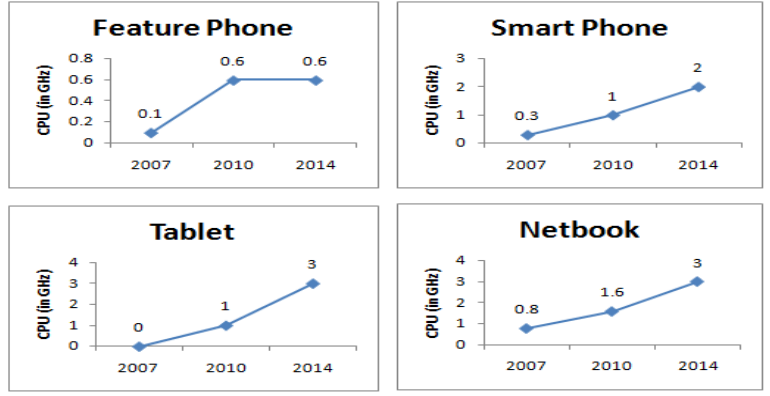
\includegraphics[scale= 0.4]{figuras/comparacao_cpu.png}
    \caption{Comparação baseada na velocidade de processamento}
    \label{comparacaoCPU}
  \end{figure}
  
  \begin{figure}[ht]
    \centering
    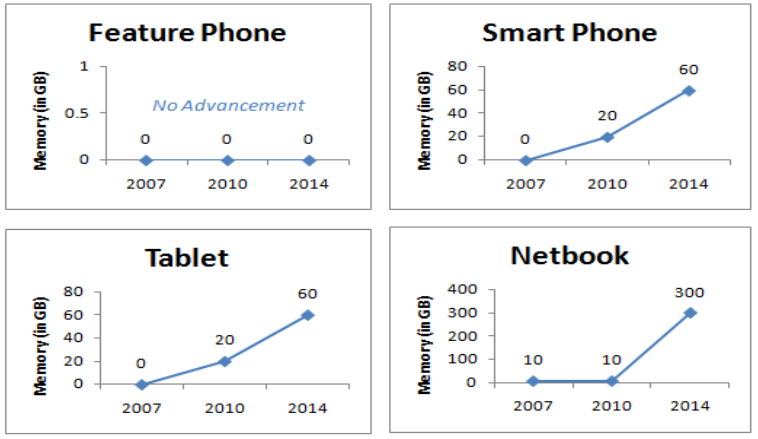
\includegraphics[scale= 0.4]{figuras/comparacao_hd.png}
    \caption{Comparação baseada na capacidade de armazenamento}
    \label{comparacaoHD}
  \end{figure}
  
  
  \item \textbf{Disponibilidade da rede:}
  
  O MCC deve garantir que haja conectividade rápida e contínua com a Internet. O dispositivo móvel está sempre
  ligado à nuvem a partir de qualquer lugar e hora que o usuário precisar. 
  Uma nova tecnologia que oferece uma solução para armazenamento em cache de dados utilizando um dispositivo móvel é o HTML5.
  Isso permite que o aplicativo da nuvem continue executando, mesmo que haja alguma interrupção na conexão \cite{alizadeh2013}.
  
  \item \textbf{Largura de banda da rede:}
  
  Um requisito importante da MCC é que a comunicação seja contínua e consistente, porém, as redes sem fio 
  estão alinhadas com espaço de transmissão de baixa largura de banda, intermitente e menos confiável 
  em comparação com redes que estão conectadas\cite{alizadeh2013}.
  
  \item \textbf{Questões de Segurança:}
  
  O principal desafio de usar o MCC é a segurança dos dados. 
  Devido ao avanço da tecnologia, os riscos de segurança de dados também aumentam.
  Todos querem proteger seus dados privados e regulamentados.
  Existe a necessidade de segurança não só no dispositivo móvel, mas também no sistema de armazenamento baseado em nuvem \cite{kumar2014}.
  
  \item \textbf{Dificuldades na implementação de PaaS e IaaS no MCC:}
  
  O MCC é uma técnica de computação multiplataforma devido à disponibilidade de diferentes plataformas em diferentes 
  dispositivos móveis. Então, PaaS é difícil de implementar. Os dispositivos móveis também não possuem nenhuma 
  infra-estrutura apropriada para usar o IaaS. Então, o MCC é limitado ao modelo de serviço da nuvem SaaS \cite{kumar2014}.
  
  % \item \textbf{Eficência de acesso a dados:}

  
\end{enumerate}


\section{Considerações Finais}

\bibliographystyle{abbrv}
\bibliography{article}

\end{document}
